\documentclass[10pt,twocolumn,letterpaper]{article}

\usepackage{cvpr}
\usepackage{times}
\usepackage{epsfig}
\usepackage{graphicx}
\usepackage{amsmath}
\usepackage{amssymb}
\usepackage{booktabs}
\usepackage{floatrow}

% Include other packages here, before hyperref.

% If you comment hyperref and then uncomment it, you should delete
% egpaper.aux before re-running latex.  (Or just hit 'q' on the first latex
% run, let it finish, and you should be clear).
\usepackage[breaklinks=true,bookmarks=false]{hyperref}

\cvprfinalcopy

\def\cvprPaperID{****} % *** Enter the CVPR Paper ID here
\def\httilde{\mbox{\tt\raisebox{-.5ex}{\symbol{126}}}}

% Pages are numbered in submission mode, and unnumbered in camera-ready
%\ifcvprfinal\pagestyle{empty}\fi
\setcounter{page}{1}
\begin{document}

%%%%%%%%% TITLE

\title{
	Histogram Approach: Deep Learning Texture Analysis}


\author{SSTP Participant\\
Tyler (Taewook) Kim\\
Kent School\\
1 Macedonia Rd, Kent, CT 06757\\
{\tt\small kimt20@kent-school.edu} 
% For a paper whose authors are all at the same institution,
% omit the following lines up until the closing ``}''.
% Additional authors and addresses can be added with ``\and'',
% just like the second author.
% To save space, use either the email address or home page, not both
\and
Graduate Research Assistant\\
Joshua Peeples\\
University of Florida\\
1064 Center Dr, Gainesville, FL 32611\\
{\tt\small jpeeples@ufl.edu}
}

\maketitle
%\thispagestyle{empty}

%%%%%%%%% ABSTRACT
\begin{abstract}
   The ABSTRACT is to be in fully-justified italicized text, at the top
   of the left-hand column, below the author and affiliation
   information. Use the word ``Abstract'' as the title, in 12-point
   Times, boldface type, centered relative to the column, initially
   capitalized. The abstract is to be in 10-point, single-spaced type.
   Leave two blank lines after the Abstract, then begin the main text.
   Look at previous CVPR abstracts to get a feel for style and length.
\end{abstract}

%%%%%%%%% BODY TEXT

%-------------------------------------------------------------------------
\section{Introduction}
 Texture analysis is a process of characterizing texture in an image by spatial variation in pixel intensity values or gray levels. Image texture is a complex visual pattern that is one of the crucial sources of visual information. Some of the texture properties include but not limited to perceived lightness, uniformity, density, roughness, and granulation \cite{Materka98textureanalysis}. This field has been one of the popular research topics in computer vision and machine learning due to its broad impact on numerous fields \cite{Cavalin2017methods}. In medical imaging, texture analysis can quantify the tumor heterogeneity based on MRI, CT, or PET images. \cite{Nalepa2014medical} In \cite{Pinto2016agri}, researchers implement texture analysis based on leaf images to classify various crop diseases.
\\

 Approaches to texture analysis are categorised into four approaches: structural, statistical, model-based, and transform. {\bf Structural analysis} represent texture by microtexture and macrotexture based on pre-defined primitives and the placement rules. {\bf Statistical approaches} represent texture indirectly with methods such as analyzing statistics given by pairs of pixels. {\bf Model-based texture analysis} interprets an image texture using fractal and stochastic models. Lastly, the {\bf transform methods} of texture a nalysis use methods such as Fourier, Gabor, and Wavelet transforms to interpret texture characteristics such as frequency or size. \cite{Materka98textureanalysis}


%-------------------------------------------------------------------------


\subsection{Related Works}


\par Texture analysis is similar to object recognition but it differs because spatial relationships of patterns in the image are important for most texture analysis approaches, as opposed to points of interests for object recognitions \cite{Cavalin2017methods}. Texture-based datasets also have higher dimensionality compared to simple color and shape-based datasets used in object recognition, which makes it a harder task \cite{Basu2018deeptexture}. In order to confront the complexity of texture datasets, several different methods to perform texture analysis have been proposed throughout the literature.
\\


%Traditional Approach
 One of the previous approaches is a traditional feature approach where researchers used different texture descriptors to observe the region homogeneity and the histograms of these region borders. In \cite{Basu2018deeptexture}, the authors present a review of various hand-crafted features including traditional texture descriptors such as Local Binary Patterns (LBP)\cite{Ojala2002lbp} and Gray-Level Co-Occurrence Matrices (GLCM)\cite{Haralick1973GLCM} as well as a patch- and multiscale-based approaches. These methods have been used for the past decades and have proved their effectiveness in various applications. 
 \\
 
 %DL Approach
 With the recent advances on Convolutional Neural Networks (CNN), researchers have applied deep neural networks to improve performance and avoid the laborious process of developing hand-crafted features. Rather than manually designing features for the machine learning model, deep learning approaches are capable of automatically extracting features from labeled datasets and yield higher performance. However, deep neural networks such as Convolutional Neural Network (CNN) require a copious amount of labeled data along with immense amounts of processing power. 
\\


%Combined Approach
In recent years, there have been several studies where researchers combined the deep learning approach and traditional hand-crafted features to create a hybrid model. 
Nguyen et al. \cite{Nguyen2018Face} proposed a new presentation attack detection (PAD) method that uses (CNN)  and the multi-level local binary pattern (MLBP) method together to form a hybrid feature with a higher discrimination ability. In \cite{Nijhawan2019snowmap}, the authors proposed a hybrid model which can learn from both deep learning features derived from spectral data as well has hand-crafted features derived from synthetic aperture radar (SAR) imagery and elevation. Some of these hybrid models do not require an immense amount of labeled data but combine automated feature learning and traditional hand-crafted feature to improve performance \cite{Nijhawan2019snowmap}. 
Zhang et al., proposed a Deep Texture Encoding Network where they added an encoding layer on top of convolutional layers \cite{Zhang2016ten}. This model was able to learn convolutional features and encoding representation simultaneously. A theoretical analysis was on implementing deep neural networks specifically for texture classification purposes was conducted to demonstrate the need for the integration of traditional and neural features \cite{Basu2018deeptexture}. These pioneering attempts showed improved performance compared to previous methods with deep learning algorithms or hand-crafted features alone. 

There were also papers which focused on implementing histogram layers for various applications. 
In \cite{Sedighi2017steg}, the authors added a histogram layer to the CNN to mimic existing features such as projection spatial rich model (PSRM) and proposed the model for steganalysis applications. By implementing a new histogram layer, they were able to capture the statisctics from the feature maps with the histogram layer. Wang et al \cite{Wang2018learnable} proposed a learnable histogram layer that can backpropagate errors as well as learn the optimal bin centers and widths. Two architectures were developed for object detection and semantic segmentation, and both models were able to achieve high performance.
However, previous studies were limited to using global histograms which caused loss in spatial information. They were also limited to using a single histogram layer.

%-------------------------------------------------------------------------
\subsection{Goal of Research}

In this paper, we propose a novel model that incorporates a localized histogram layer for convolutional neural  networks (CNNs). Our studies will be the first attempt to implement such a hybrid model for texture analysis applications and implementing localized histograms will provide several advantages.
1) Spatial information, which is important for texture, will be retained as opposed to previous global methods. 2) Our approach will use radial basis functions (RBFs) which will relax the binning constraint because each feature value's contribution will be based on their proximity to each bin center and associated bin width. Additionally, this will enable the network to be less sensitive to various outliers and ambiguity in the data. 3) This architecture will allow a differentiable histogram operation for deep learning algorithms as well. 4) Lastly, our model will have a stackable histogram layers which is capable of capturing more higher-level features.
\\




\section{Methodology}
%------------------------------------------------------------------------

\subsection{Binning Operation}

Binning operation in standard histogram can be expressed with the following counting fuction:
\begin{equation}
\label{eqn:cf}
y_k = \begin{cases}
1,B_k - w \leq x_k < B_k + w\\
0, otherwise
\end{cases}
\end{equation}

This indicator function returns "1" if the  element falls into a bin and returns "0" else. The condition when an element falls into a bin is defined by $B_k - w \leq x_k < B_k + w$, $B_k$ being the bin center and $w$ being the bin width. However, the standard histogram operation is not differentiable and cannot be used for the backpropagation.\\

Therefore, our approach is to perform a localized binning operation with a sliding window. RBFs will be used instead of standard histogram operation to approximate the count values:


\begin{equation}
\label{eqn:rbf}
y_k =
\cfrac{1}{MN}\sum_{i=1}^{M}\sum_{j=1}^{N}e^{-\cfrac{\left(x_{ij}-\mu_k\right)^2}{\sigma_k^2}}.
\end{equation}


The equation \ref{eqn:rbf} returns the count $y_k$, for kth bin center $\mu_k$ and width $\sigma_k$ from the feature map value $x_{ij}$ .


An example with M$\times$N window in an image is shown in Figure \ref{fig:3_1_1}. Each square represents a pixel with a single intensity value of 1, 2, or 3. Every pixel will contribute to every bin but not equally due to the RBF we are using.

\begin{figure}
	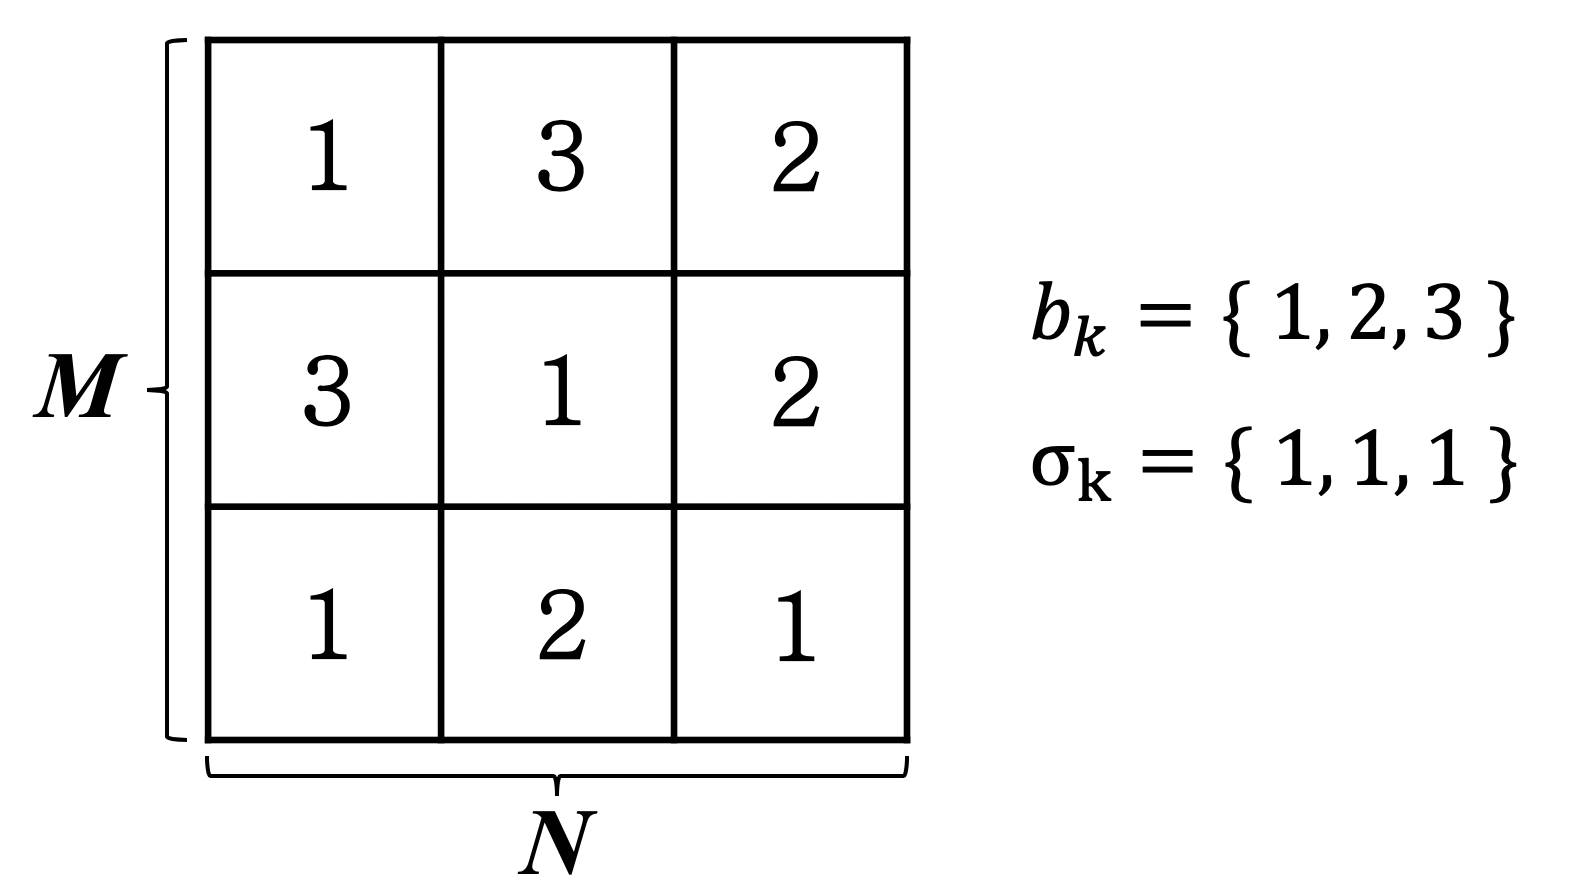
\includegraphics[width=1.0\linewidth]{./Images/3_1_1.png}
	\caption{M$\times$N Window}
	\label{fig:3_1_1}
\end{figure}

\begin{table}
	\begin{tabular}{cccc}
		\hline
		\textbf{} & \textbf{\begin{tabular}[c]{@{}c@{}}$b_0$\\ Value: 1\end{tabular}} & \textbf{\begin{tabular}[c]{@{}c@{}}$b_1$\\ Value: 2\end{tabular}} & \textbf{\begin{tabular}[c]{@{}c@{}}$b_2$\\ Value: 3\end{tabular}} \\ \hline
		Standard & 0.44 & 0.33 & 0.22 \\ \hline
		RBF & 0.57 & 0.42 & 0.35 \\ \hline
	\end{tabular}
	\caption{Normalized Frequency Comparison}
	\label{tab:table1}
\end{table}

Table \ref{tab:table1} compares the resulting count value from the two equations introduced. Each column represents the bins, $b_0$, $b_1$ and $b_2$ each indicating bin center of 1, 2, and 3 respectively. The first row shows the value calculated by \eqref{eqn:cf} with $w = 0$, and the second row is based on \eqref{eqn:rbf}. RBF is used to approximate the counting function because it allows differentiation thereby allowing the model to learn via backpropagation. As shown in Figure \ref{fig:3_1_1}, $\sigma_k$ is set to be 1, which makes the difference between the two values larger. $\sigma_k$ is a crucial factor that determines this difference. As $\sigma_k$ value becomes smaller, the model will only consider the values that are very close to the bin center. If model learns the optimum $\sigma_k$ value, we will be able to account for ambiguity in the data as opposed to crisp histograms. As $\sigma_k$ value becomes larger, every element will fall into the same bin.

\subsection{Experiment Design}

\begin{figure}
	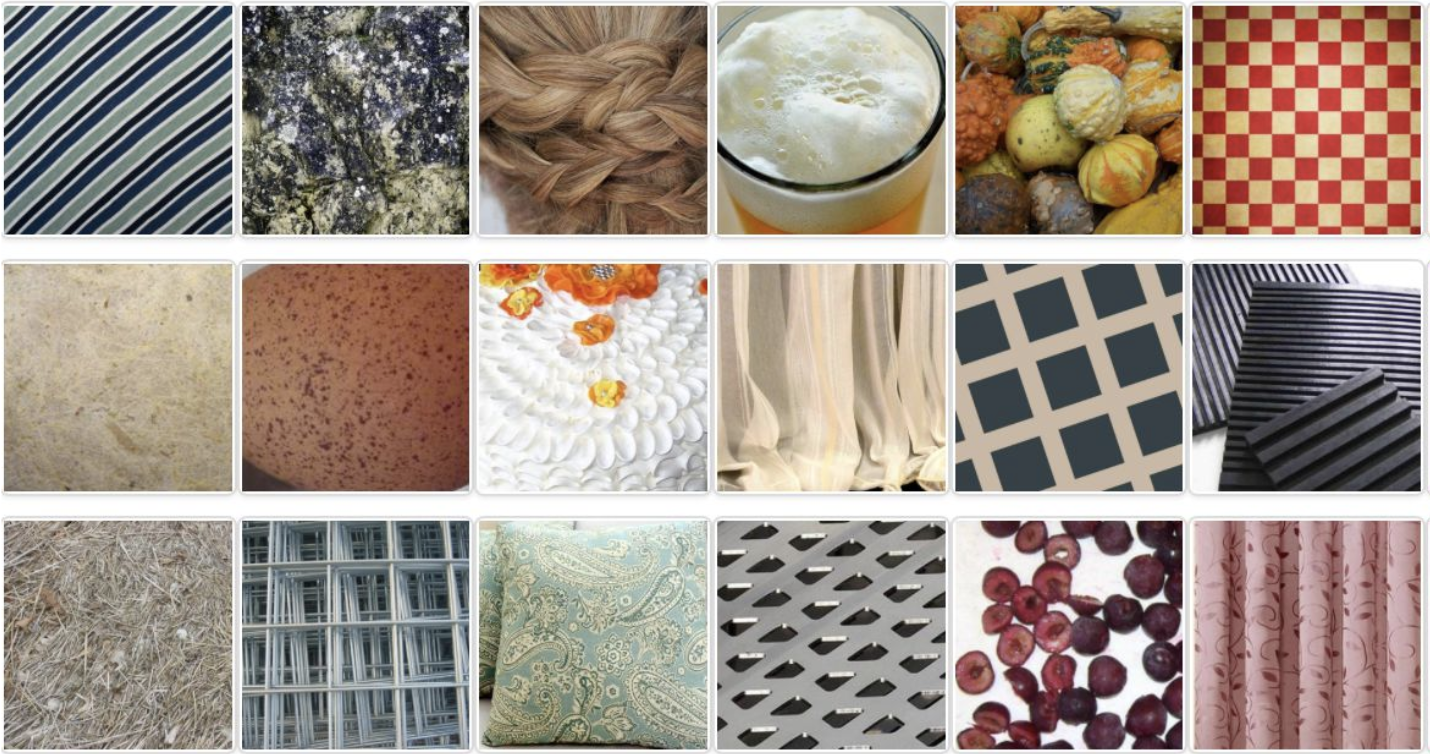
\includegraphics[width=1.0\linewidth]{./Images/3_2_1.png}
	\caption{Example of DTD Images \cite{cimpoi14DTD}}
	\label{fig:3_2_1}
\end{figure}

To evaluate the performance of the proposed model, we used Describable Textures Dataset (DTD), a texture database with 5640 images classified into 47 categories. We will use five different artificial neural networks (ANN) that are comprised of convolutional and histogram layers to classify the images. We will compare the results both quantitatively and qualitatively. In qualitative analysis, we will focus on displaying images that are classified correctly or incorrectly by each network. In quantitative analysis, we record accuracy(class and overall), class precision, class recall, class F1 score, learning curve, and confusion matrices.

\subsection{Training Procedure}
For our training procedure, our data is first scaled to between 0 and 1. Next, we wanted to look at the effects of preprocessing our data through standardization

\begin{equation}
\label{eqn:std}
Z = \dfrac{x - \mu}{\sigma}.
\end{equation}

The equation \ref{eqn:std} represents the standardization operation, where $x$ is the original feature value, $\mu$ is the mean of that feature value, $\sigma$  is its standard deviation, and $Z$ is the resulting standardized data. 
For our dataset, $x$ is the RGB value for each pixel and the corresponding mean ($\mu$) and standard deviation ($\sigma$) for each channel will be used to normalize the data through equation \ref{eqn:std} . Data preprocessing is considered to be one of the most important components of training the model, and we want to compare the results from standardizing the data and relating this to the performance of each network. \\


For the training process, we use the same data augmentation and optimization technique for the six different neural networks. Similar to \cite{Xue2018dep}, all the samples were first resized to 256 $\times$ 256 then a crop of random size (0.8 to 1.0) of the original size and a random aspect ratio (3/4 to 4/3) of the original aspect ratio is extracted. This crop is finally resized to 224$\times$224 and horizontal flips ($p=0.5$) were used. The experiment starts with learning rate of 0.01 and batch size of 128. Throughout 100 total epochs, the learning rate decays by factor of 0.9 for every 10 epochs. During the learning rate decay, Adam, an adaptive learning rate optimization algorithm, is used. Adam allows for efficient stochastic optimization that only requires first-order gradients, allowing for little memory requirement\cite{Kingma2014adam}. 



{\small
\bibliographystyle{ieee_fullname}
\bibliography{egbib}
}

\end{document}
